\chapter{Evaluation and Measurement}
In the previous chapters, we showed our modification to \dpy keeps backward compatibility and extends the semantics. In this chapter, we show the performance measurement based on several tasks and platforms to demonstrate the usability of our modification.

We demonstrate on two kinds of workflows: the prime sieve and the cross-correlation, both have been discussed in the Use Cases chapter. The cross-correlation workflow is from the previous \dpy paper and is largely computation-intensive. We expect to demonstrate the overhead of \tincdep is quite small compared to the actual computational job, and therefore can be neglected. The prime sieve was shown above (both in \ref{sec:uc_sieve} and \ref{sec:dynexp_example}) and is not computation-intensive. We use it to show \tdynexp works correctly and the benefit \tdynexp brings. We also use several static version prime sieves (constructed using the old semantics) to measure the scalability of \tincdep as they virtually involve no computation but demonstrate the overheads of communication.

To show the performance and perform evaluation, we describe here what platforms we choose to perform the measurement. Because this is an MSc project, except for my laptop, we use two shared-resource platforms (clusters) to perform our measurement: the teaching cluster of the School of Informatics (InfCluster) and the university's cluster (EDDIE).
The configurations of the machines vary among all nodes in the clusters, but each cluster has some typical configurations. They are listed in Table \ref{tbl:list_measurement}.

\begin{table}[h]
\centering
\begin{tabular}{|c|c|c|c|}
\hline
 & Laptop & InfCluster & EDDIE \\ \hline
CPU (module) & Intel Core i7 5500U & Intel Xeon E5 2650 (v3,v4) & Intel Xeon E5 2630 v3 \\ \hline
CPU (cores) & 4 & 32, 40, 48 & 16 \\ \hline
RAM (GB) & 8 & 64 & 64, 128 \\ \hline
\end{tabular}
\caption{Typical configurations of measurement platforms. Cores means virtual cores which is $num\_cores \times num\_threads\_per\_core$.}
\label{tbl:list_measurement}
\end{table}

The EDDIE cluster restricts users to use only multiples of 16 as the number of cores. It also restricts us to use at most the same number of cores the number of MPI processing elements, so we can't measure large sieves on it. The Laptop is not powerful enough (no enough RAM) to run sensible cross-correlations so we exclude it from the measurement of cross-correlations.

We use several different workflows and configurations to test different aspects of the system's performance. For cross-correlation (see Table \ref{tbl:list_measurement_xcorr}), we vary the number of nodes and the number of traces and duration of data to see how performance changes. For the prime sieve, we use several different ranges, both the static version and the dynamic version, to test the correctness of our system (see Table \ref{tbl:list_measurement_sieve}). We also vary the number of initial nodes (\ie the ``np'' parameter) for the dynamic version to see how time consumption change. For each measurement, we run the same configuration for several (7 or more) times to get a more typical performance.

\begin{table}[h]
\centering
\begin{tabular}{ccccccccc}
\hline
Platform & \multicolumn{6}{c}{EDDIE} & \multicolumn{2}{c}{InfCluster} \\ \hline
Duration & \multicolumn{4}{c}{90 days} & \multicolumn{2}{c}{1 hour} & \multicolumn{2}{c}{90 days} \\
Traces & \multicolumn{2}{c}{4} & \multicolumn{2}{c}{2} & \multicolumn{2}{c}{400} & 4 & 2 \\ \hline
Processes & 16 & 32 & 16 & 32 & 16 & 32 & 32 & 32 \\ \hline
\end{tabular}
\caption{Different options used to run the measurement of cross-correlation.}
\label{tbl:list_measurement_xcorr}
\end{table}

\begin{table}[h]
\centering
\begin{tabular}{|c|c|c|c|c|}
\hline
Platform & \multicolumn{2}{|c|}{InfCluster} & \multicolumn{2}{|c|}{Laptop} \\ \hline
Max number & 100 & 1000 & 100 & 1000 \\ \hline
Number of sieves & 26 & 168 & 26 & 168 \\ \hline
np (dynamic only) & \multicolumn{4}{|c|}{3 \quad 8 \quad 13} \\ \hline
\end{tabular}
\caption{Different options used to run the measurement of \tdynexp using the prime sieve. The variation of the ``np'' parameter is only used when using the dynamic version (\ie with \tdynexp) of \dpy.}
\label{tbl:list_measurement_sieve}
\end{table}

The cross-correlation workflow is used to demonstrate how \tincdep affects overall performance in a production environment because it is computation-intensive. The comparison between the static prime sieve workflow and the dynamic prime sieve workflow is used to show the performance of \tdynexp, but is unlikely to demonstrate anything about \tincdep in production because the amount of computation is significantly small. We also run several different options of the static prime sieve (see Table \ref{list_measurement_sieve_static}) under the \dpy system with and without \tincdep with just enough number of processes to measure the overhead of communication introduced by \tincdep.

\begin{table}[h]
\centering
\begin{tabular}{ccccccccc}
\hline
Platform & \multicolumn{8}{c}{InfCluster} \\ \hline
\multirow{2}{*}{Cores} &
\multicolumn{3}{c|}{32} \\ \cline{2-9}
& \multicolumn{8}{c}{128} \\ \hline
Max number & 100 & 1000 & 2000 & 3000 & 4000 & 5000 & 6000 & 7000 \\ \hline
Number of sieves & 26 & 168 & 303 & 430 & 550 & 669 & 783 & 900 \\ \hline
\end{tabular}
\caption{Different options used to run the static prime sieve for both systems (with and without \tincdep).}
\label{tbl:list_measurement_sieve_static}
\end{table}

\section{Incremental deployment}
The working process of \tincdep was described in \ref{sec:incdep_example} and the correctness was also shown there. This section focuses on the performance issues.

As said above, we use the cross-correlation workflow (xcorr) as the main workflow to demonstrate the performance. We run the workflows under different configurations, as describe above. Generally, for both workflows, we use one more node for the \tincdep version, which is required because of the mechanism of \tincdep and is an unavoidable overhead. One exception is when we reach the maximum number of cores requested on EDDIE: we only use as many as the number of cores for the number of nodes because of the restriction of the platform. To make it easier to read, we show only the number of worker nodes for \tincdep -- by subtracting $1$ from the number of nodes\footnote{However this will lead to misalignment when the number of processes is the same as the number of cores on EDDIE, which is \textbf{not} a mistake or error.}. We present the results in Figure \ref{fig:xcorr_infcluster}, \ref{fig:xcorr_infcluster_90_2}, \ref{fig:xcorr_eddie} and \ref{fig:xcorr_eddie_400}.

\begin{figure}[h]
\centering
\begin{minipage}{\textwidth}
    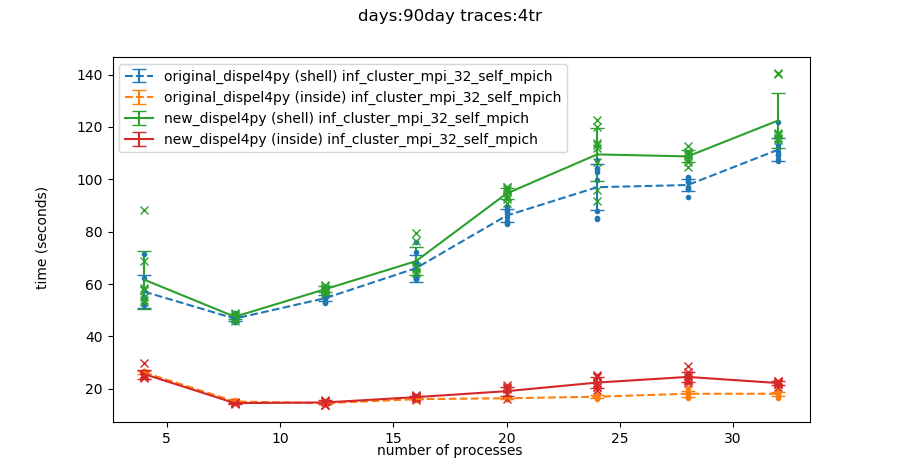
\includegraphics[width=1\textwidth]{figures/xcorr_infcluster_90day_4tr}
    \caption[Caption for LOF]%
      {Execution time of XCorr (without plotting) on InfCluster with 4 traces of length 90 days\footnote{The period of time for which the seismic trace was recorded.}.}
\label{fig:xcorr_infcluster}
\end{minipage}
\end{figure}

\begin{figure}[h]
\centering
    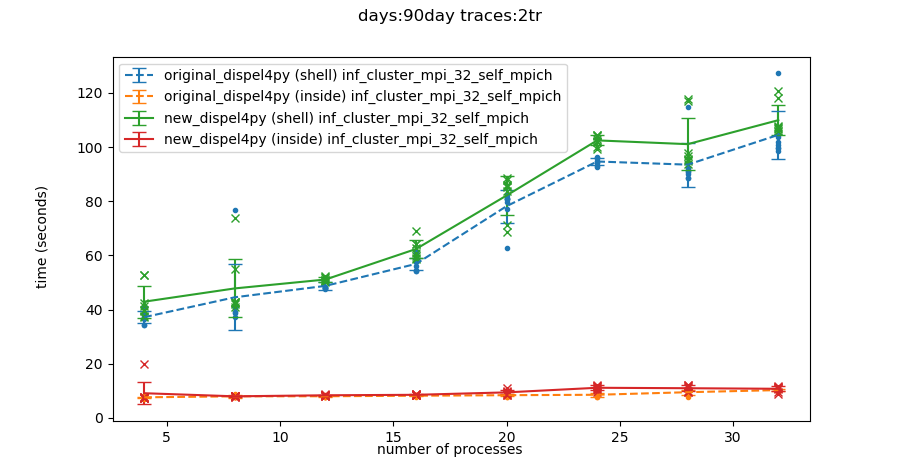
\includegraphics[width=0.9\textwidth]{figures/xcorr_infcluster_90day_2tr}
\caption{Execution time of XCorr (without plotting) on InfCluster with 2 traces of length 90 days.}
\label{fig:xcorr_infcluster_90_2}
\end{figure}

\begin{figure}[h]
\centering
    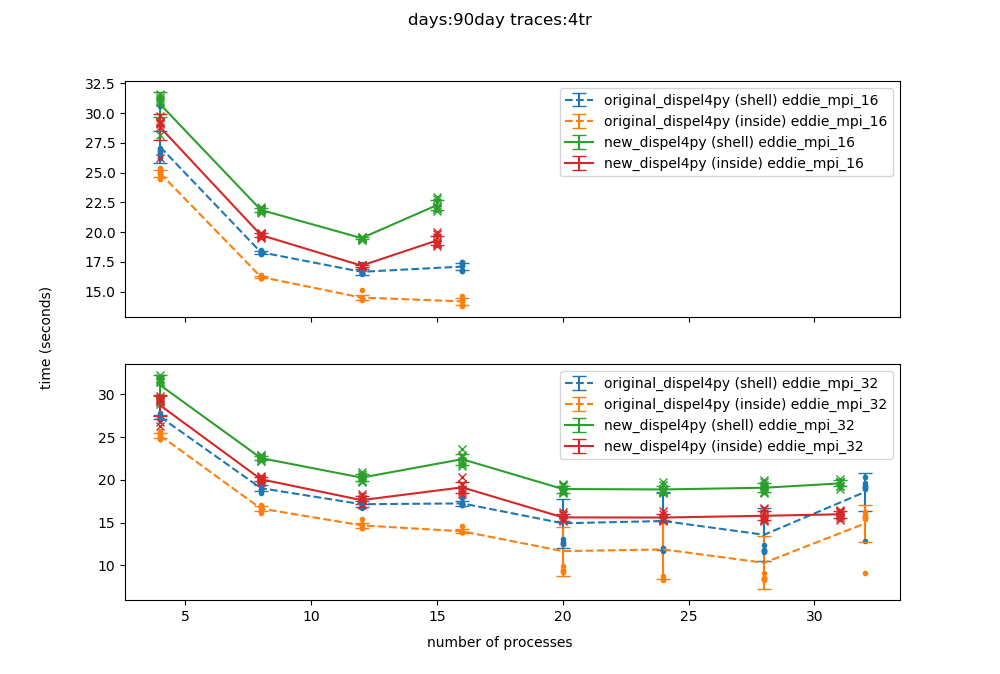
\includegraphics[width=1.10\textwidth]{figures/xcorr_eddie_90day_4tr}
\caption{Execution time of XCorr (with plotting) on EDDIE with 4 traces of length 90 days.}
\label{fig:xcorr_eddie}
\end{figure}

\begin{figure}[h]
\centering
    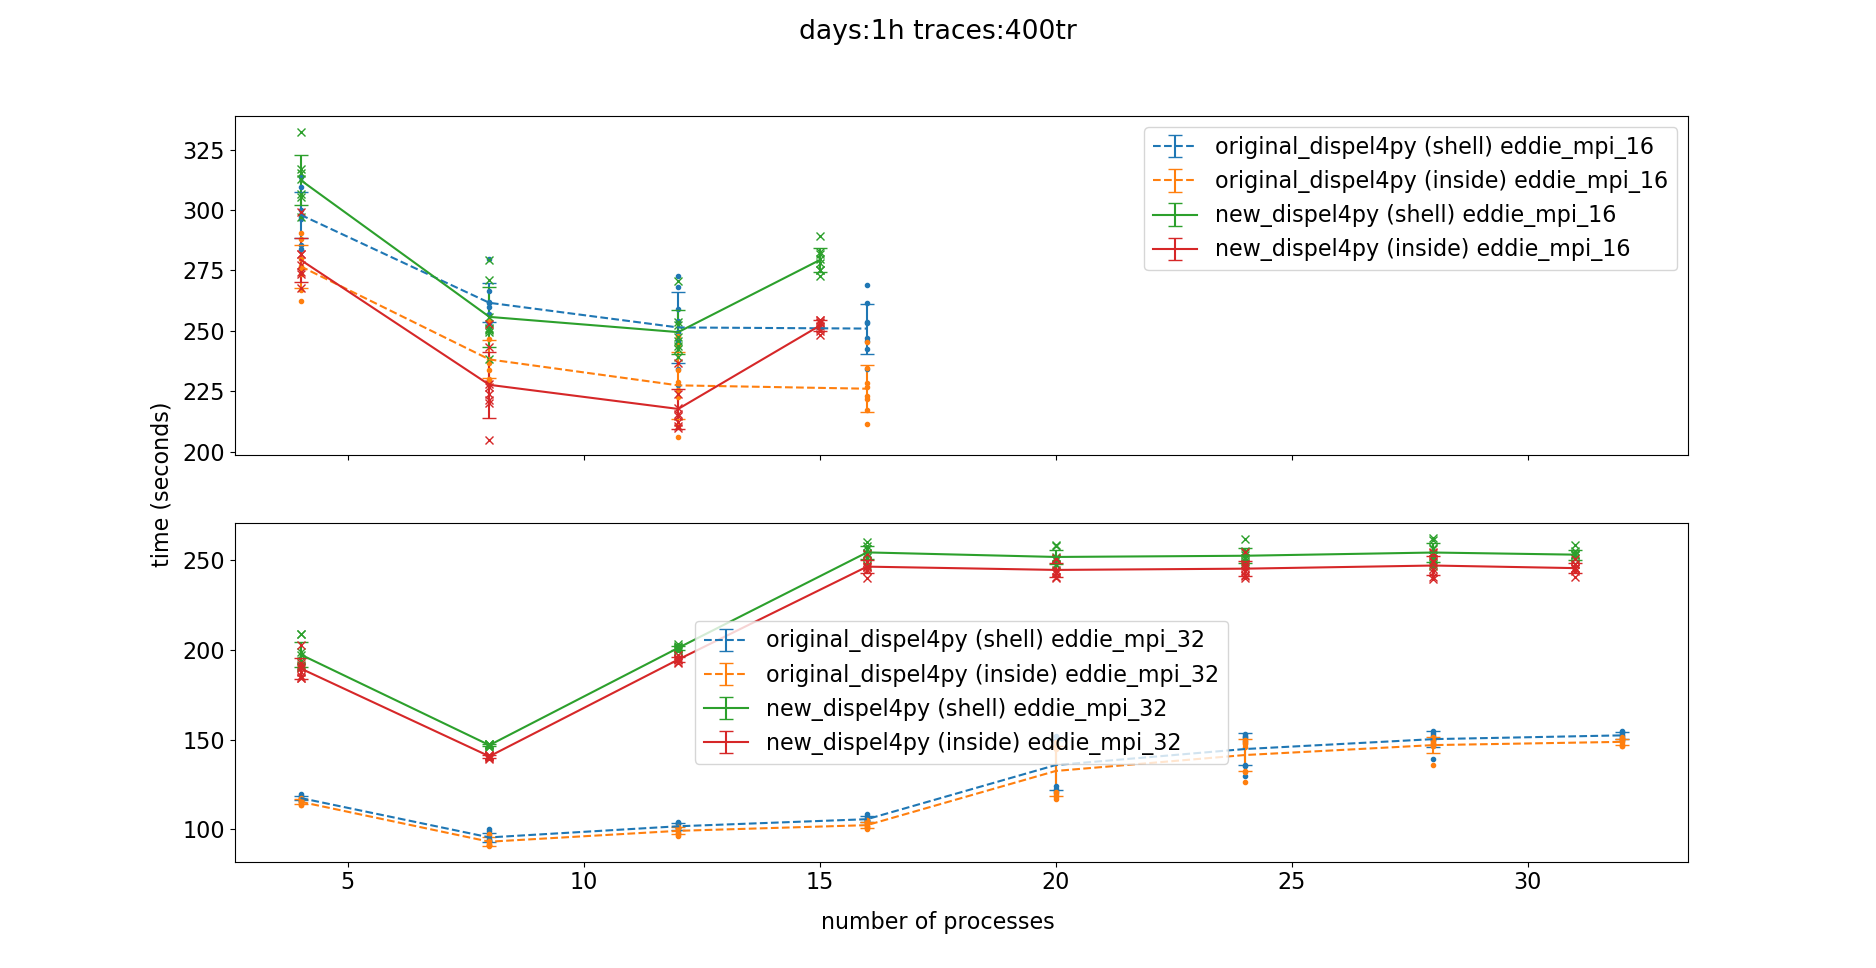
\includegraphics[width=1\textwidth]{figures/xcorr_eddie_1h_400tr}
\caption{Execution time of XCorr (without plotting) on EDDIE with 400 traces of length 1 hour.}
\label{fig:xcorr_eddie_400}
\end{figure}

To better explain and show some of the behaviours or properties, we also performed a set of measurements on the InfCluster with the static version of the prime sieve workflow. We used static numbers of processes (\emph{just enough} to execute the job) for both the original system and the new system. The results are shown in Figure  \ref{fig:sieve_static_32} and \ref{fig:sieve_static_128}.

\begin{figure}[h]
\centering
    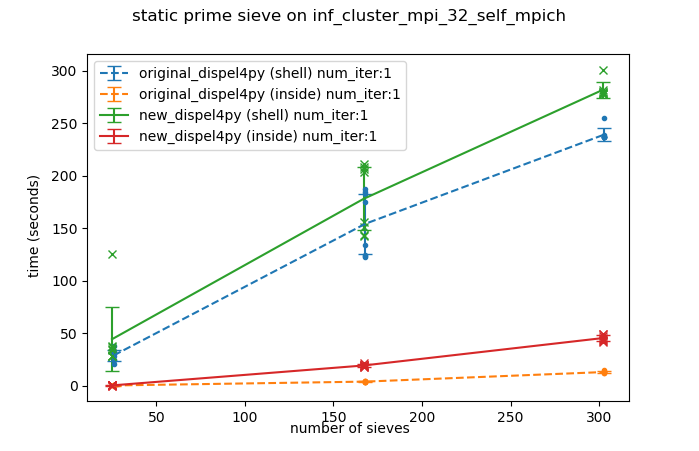
\includegraphics[width=0.8\textwidth]{figures/sieve_static_32}
\caption{Static sieves executed by both the original and the new version of \dpy on InfCluster with 32 cores.}
\label{fig:sieve_static_32}
\end{figure}

\begin{figure}[h]
\centering
    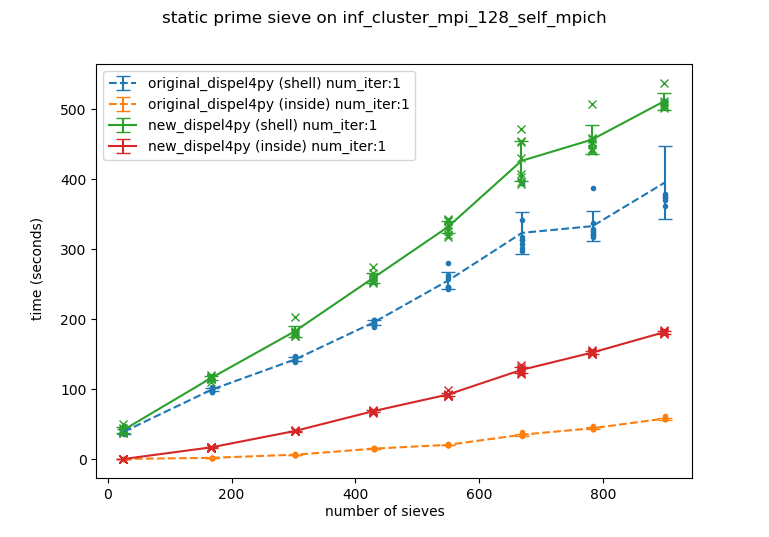
\includegraphics[width=0.8\textwidth]{figures/sieve_static_128}
\caption{Static sieves executed by both the original and the new version of \dpy on InfCluster with 128 cores.}
\label{fig:sieve_static_128}
\end{figure}

We explain here the notations in the figures:
\begin{itemize}
	\item The top of each figure is two of the configuration options: the number of traces and the duration of the data collected from.
	\item The dashed lines shows data / performance from the original version of \dpy; the solid lines shows data from our modifications of \dpy.
	\item The dots (whether they are points or crosses) represent individual performance data of the line with the same colour.
	\item The errorbar shows one standard deviation away from both sides of the mean.
	\item In the legends, there are several sections in the texts.
	\begin{enumerate}
		\item The first section is the system version we used; 
		\item The second section (wrapped in parentheses) shows the recording method of time and defaults to \textbf{shell} when omitted.
		\item The third section shows the platform and the number of cores requested to perform this measurement, and there may be some additional information (useful for us, but not for the readers).
	\end{enumerate}
\end{itemize}

In the figures, we show two different recordings of time: one is inside the program (notated as \textbf{inside}) and the other is outside the program (noted as \textbf{shell}). The reason we use two recordings is that we want to also investigate the time consumed during programme running rather than the time for both initialization and running.

We have removed some significant outliers from the data used to draw the figures. There are still some data points outside of one standard deviation but we can not sensibly remove them because they are not apparently away from other data points. These outliers could be caused by the resources used by other processes in the OS of the execution machine(s) because we are using shared-resource platforms to perform our measurement.

We can obtain much information from the figures, and we summarize them into five categories: \\\\
\textbf{Actual data processing takes significantly more time than the communication led by \tincdep}\quad
The total execution time is not significantly different from the original \dpy version and our modification (\tincdep) in all figures. The time difference is almost always constant for each configuration (\eg less than 10 seconds in Figure \ref{fig:xcorr_eddie}) so we have confidence that it won't increase when the total execution time increases and is acceptable when using under production -- because the total execution time would be significantly longer than that in our demonstration so this small difference won't even be noticed. The difference between each two time recordings of each configurations also shows that the time consumed to initialize one extra process (for the coordinator) isn't significant. \\\\
\textbf{Inter-machine communication causes overheads}\quad
In Figure \ref{fig:xcorr_eddie_400}, the first subfigure shows the performance of \tincdep matches the performance of the old system, and increasing parallelization increases performance in its range. However, in the second subfigure, the total execution time rises when the number of processes increased from 8 to 12 and never went down with increasing of the number of processes. We believe this is because of inter-machine communication -- each machine in EDDIE consists of 16 cores so we are actually using 2 machines when requesting 32 cores (which is the case of the second subfigure). \\\\
\textbf{Synchronization causes overheads}\quad
In the second half of Figure \ref{fig:xcorr_eddie} when the number of processes is larger than needed, our version of system consumes almost constant time while the original version varies much. We define \emph{needed} as: processes are just enough to fully parallelize the computation. Because of the definition of the cross-correlation workflow, the number of cross-correlation is $C^2_n$ \footnote{Also denoted as $\binom{n}{k}$.} for $n$ traces where $C^k_n$ represents the number of $k$ combinations in $n$ elements. This leads to $1+C^2_n \cdot 2$ processes for $n$ traces when the workflow does not contain the plotting step and $1+C^2_n \cdot 2$ when the workflow contains the plotting step. For 2 traces, the number of needed processes is 3 (or 4 if including plotting); for 4 traces, the number of needed processes is 13 (or 19 if including plotting).

We argue this is because of our strategy of using \lstinline|comm.Barrier()| to synchronize and record time (which is what we added to the original version of \dpy) -- it performs a full synchronization and takes more time compared to our one-sided communication (only the coordinator sends signals to workers) in \tincdep.

This also explains the increasing of time consumption at the tail of the first subfigure of Figure \ref{fig:xcorr_eddie} and \ref{fig:xcorr_eddie_400} -- extra processes are spawned and synchronized but not used to parallelize the computation (because they are not enough to form a complete partition). They form a pure overhead without any benefits to the performance so the time consumption increased. \\\\
\textbf{Initialization on InfCluster is significantly slow}\quad
In Figure \ref{fig:xcorr_infcluster} and \ref{fig:xcorr_infcluster_90_2}, there are huge gaps between the time recorded inside and outside. This indicates much time is consumed during the initialization of MPI runtime, while the time for actual data computation is almost the same as the EDDIE platform (Figure \ref{fig:xcorr_eddie}). This behaviour is also demonstrated in Figure \ref{fig:sieve_static_32} and \ref{fig:sieve_static_128}. \\\\
\textbf{Increasing the number of PEs increases the overhead led by \tincdep}\quad
We can see in Figure \ref{fig:sieve_static_32} and \ref{fig:sieve_static_128} that the gap between the original version and the new version increases along with the increasing of the number of PEs (reflected by the number of sieves). As shown in the figure, this overhead grows approximately linearly. We performed a linear regression on the \textbf{inside} record of time, and the slope is about $0.15$. This shows the overhead will increase but is unlikely to ``explode''. \\

In conclusion, the time consumed between our new system with \tincdep and the original system without \tincdep is quite close especially when the total number of PEs is small. Also notice there are some compromises in our implementation so there is still space to get better performance (\ie less time consumption). We believe this won't add significant overheads to a production environment so our extension is acceptable compared to the potential benefits and future optimizations it may bring.

\section{Dynamic expansion}
\tDynexp is the new property we have added to dispel4py. We use the prime sieve as our example to demonstrate how the system performs when using \tdynexp. The details of the workflows were described in \ref{sec:dynexp_example}.

The results are shown in Figure \ref{fig:sieve_opt_100} and \ref{fig:sieve_opt_1000}. The third section of the legends (in the figures) is one of the parameters controlling the number of processes spawned at the beginning.

\begin{figure}[h]
\centering
    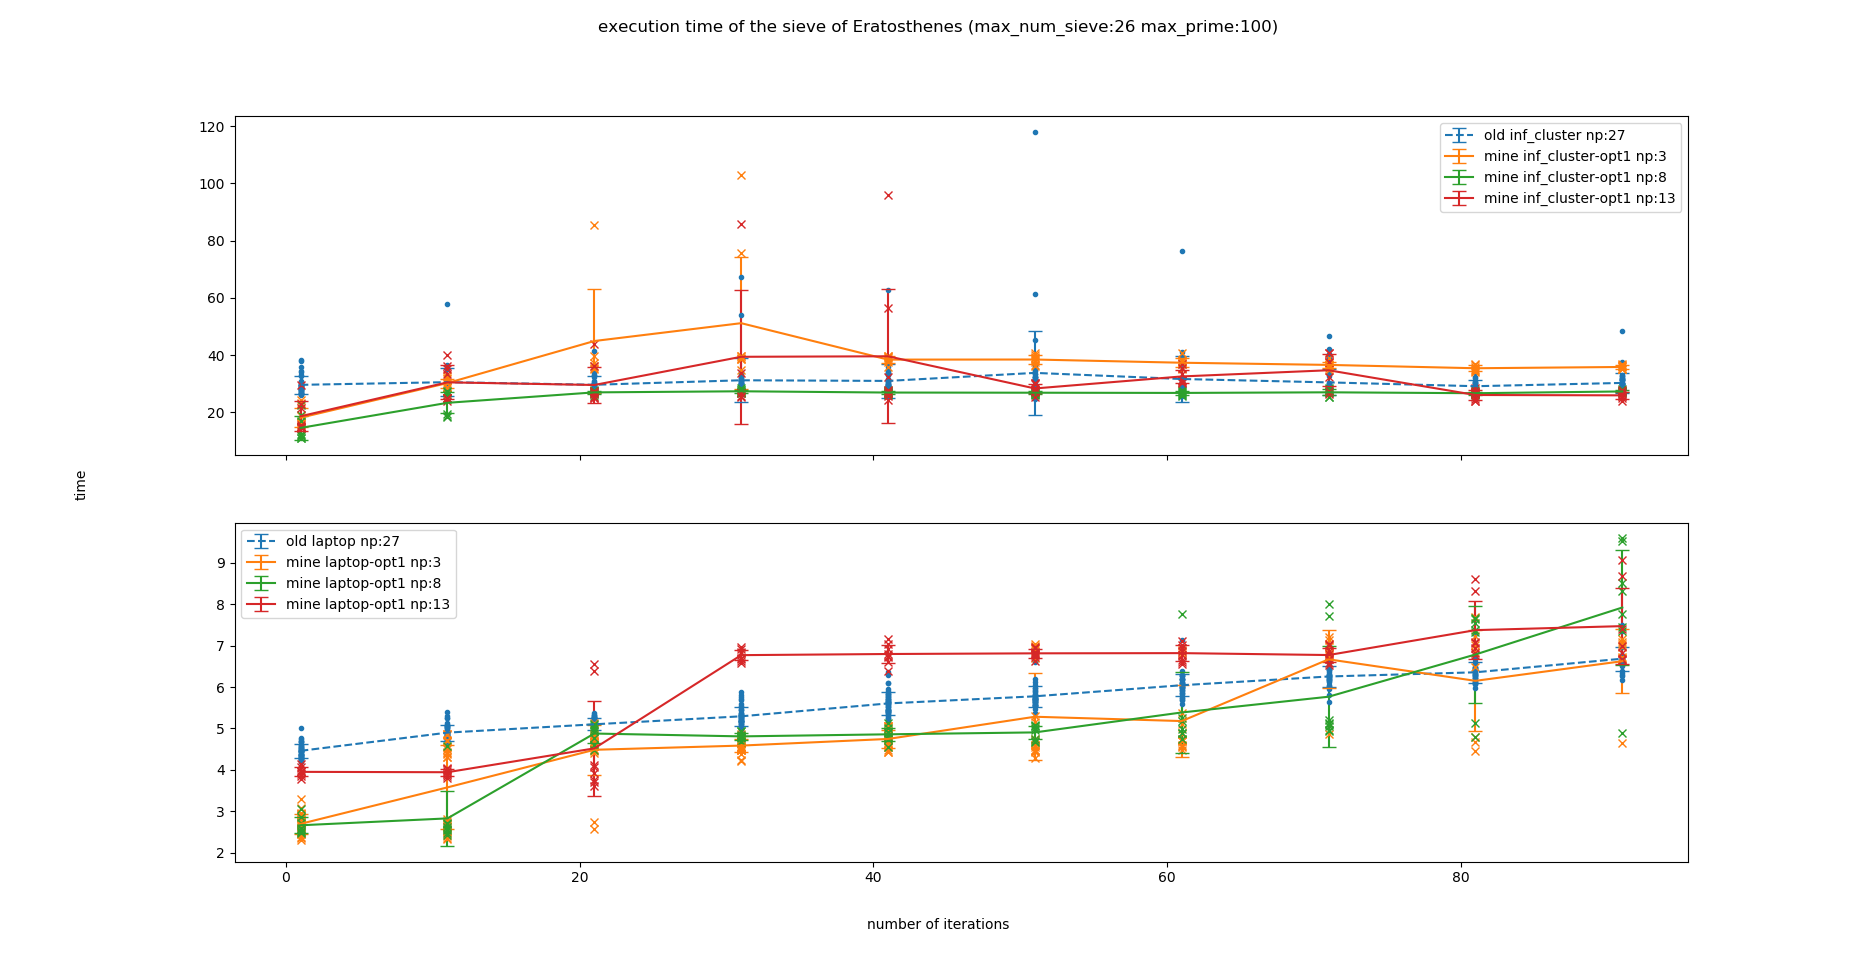
\includegraphics[width=1\textwidth]{figures/sieve_opt1_100}
\caption{Execution time of the prime sieve to find prime up to 100 on the old and new semantics.}
\label{fig:sieve_opt_100}
\end{figure}

\begin{figure}[h]
\centering
    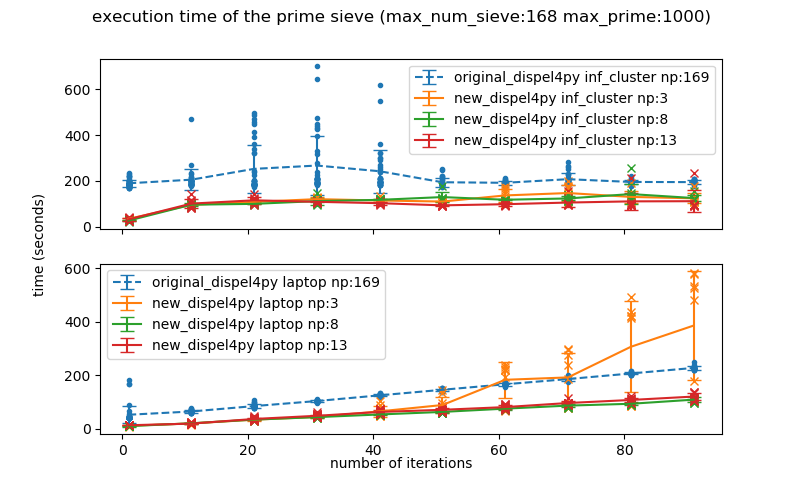
\includegraphics[width=1\textwidth]{figures/sieve_opt1_1000}
\caption{Execution time of the prime sieve to find prime up to 1000 on the old and new semantics.}
\label{fig:sieve_opt_1000}
\end{figure}

Similarly, we also removed significant outliers. The number of outliers is larger in InfCluster compared to EDDIE. This may be because the number of cores of each machine in InfCluster is larger than that of EDDIE and each machine can host more jobs, so more people are sharing the same machine. Another possible reason is because the prime sieve is not computation-intensive so the effect and latency of communication governs the performance but they are more unpredictable than the computation.

The horizontal axis in these figures is different from the previous figures (\eg Figure \ref{fig:xcorr_eddie}) -- the ``number of iterations'' means how many times the producer repeatedly produces numbers from 2 to the upper bound. One reason is because we are no longer evaluating the performance difference caused by introducing \tincdep; the other reason is we want to show the consistency of the performance -- when increasing the number of iterations, more data (numbers) go through the workflow but no more PEs are deployed or created.

As we can see in the figures, there is no significant indication of whether the dynamic version or the static version is better. We argue that this is because much time is used to initialize for MPI communication. The dynamic version spawns significantly fewer nodes in the beginning so it can start earlier and adjust during runtime (so the leftmost points always show the dynamic version performs better). 

When increasing the number of iterations, the producer node executes longer so it can not be reused before finishing producing. Therefore, the coordinator can not reuse the producer node and also other nodes, so it is forced to spawn more nodes. This (and also producing more data takes more time) explains why the time consumed in execution increases when increasing the number of iterations.

We also tried several different sets of processes spawned in the beginning for \tdynexp. The results (also shown in the figures) match our intuition: the more processes spawned in the beginning, the more time consumed to initialize (by comparing points at 1 iteration); the more processes spawned in the beginning, the less likely spawning would happen during runtime (by comparing the number of sharp performance changes of each line).

The spawning process during runtime also takes time and may be optimised (see the \rcpt{Conclusion and Future Work} chapter) in order to get better performance for the dynamic semantics.

To draw a conclusion: in both figures, we can monitor better performance at certain points for the dynamic version. We believe they are because the dynamic version reused nodes so fewer nodes were spawned in total. This matches our expectation and may open a potential future optimization: how to identify what nodes that can be reused according to the workflow.
